\documentclass[aspectratio=169,11pt]{beamer}

\usepackage{fontspec}
\usepackage{amsmath,amssymb,bm,mathtools}
\usepackage{booktabs,tabularx,array}
\usepackage{graphicx}
\usepackage{tikz}
\usetikzlibrary{arrows.meta,positioning,fit,shapes.geometric,calc}

\setmainfont{Noto Serif CJK SC}
\setsansfont{Noto Sans CJK SC}
\setmonofont{Noto Sans Mono CJK SC}
\usefonttheme{professionalfonts}

\definecolor{navy}{HTML}{183A5A}
\definecolor{teal}{HTML}{087E8B}
\definecolor{orange}{HTML}{E07A3F}
\definecolor{green}{HTML}{3E8E63}
\definecolor{red}{HTML}{B94A48}
\definecolor{ink}{HTML}{27323A}
\definecolor{muted}{HTML}{65727C}
\definecolor{pale}{HTML}{EFF5F7}
\definecolor{linegray}{HTML}{D8E1E5}

\setbeamercolor{normal text}{fg=ink,bg=white}
\setbeamercolor{structure}{fg=teal}
\setbeamercolor{frametitle}{fg=navy,bg=white}
\setbeamercolor{title}{fg=navy}
\setbeamercolor{subtitle}{fg=muted}
\setbeamercolor{block title}{fg=white,bg=teal}
\setbeamercolor{block body}{fg=ink,bg=teal!6}
\setbeamercolor{alerted text}{fg=orange}
\setbeamercolor{itemize item}{fg=teal}
\setbeamercolor{itemize subitem}{fg=orange}

\setbeamertemplate{navigation symbols}{}
\setbeamertemplate{itemize item}{\raise0.15ex\hbox{\scriptsize$\blacktriangleright$}}
\setbeamertemplate{itemize subitem}{\raise0.15ex\hbox{\tiny$\blacktriangleright$}}
\setbeamertemplate{frametitle}{%
  \vspace{0.3em}\insertframetitle\par
  \vspace{-0.35em}{\color{teal}\rule{\textwidth}{0.7pt}}
}
\setbeamertemplate{footline}{%
  \leavevmode
  \hbox{%
    \begin{beamercolorbox}[wd=.78\paperwidth,ht=2.7ex,dp=1.1ex,leftskip=1em]{author in head/foot}%
      \color{muted}\scriptsize 自适应 Hartree treecode 与 KS--SCF
    \end{beamercolorbox}%
    \begin{beamercolorbox}[wd=.22\paperwidth,ht=2.7ex,dp=1.1ex,rightskip=1em plus1fil]{date in head/foot}%
      \color{muted}\scriptsize \insertframenumber/\inserttotalframenumber
    \end{beamercolorbox}%
  }
}

\newcommand{\SCF}{\mathrm{SCF}}
\newcommand{\Har}{\mathrm{H}}
\newcommand{\mesh}{\mathcal T}
\newcommand{\norm}[1]{\left\lVert #1\right\rVert}
\newcommand{\tagdone}{\tikz[baseline=-0.5ex]\node[rounded corners=1pt,fill=green!15,text=green,inner xsep=3pt,inner ysep=1pt,font=\scriptsize\bfseries]{已完成};}
\newcommand{\tagpre}{\tikz[baseline=-0.5ex]\node[rounded corners=1pt,fill=orange!15,text=orange,inner xsep=3pt,inner ysep=1pt,font=\scriptsize\bfseries]{初步证据};}
\newcommand{\tagnew}{\tikz[baseline=-0.5ex]\node[rounded corners=1pt,fill=teal!15,text=teal,inner xsep=3pt,inner ysep=1pt,font=\scriptsize\bfseries]{新设想};}

\title{从自适应 Hartree Treecode\\到 Kohn--Sham 自洽场迭代}
\subtitle{残差控制的多速率网格与计算结构复用}
\author{研究进展与下一步设想}
\date{2026 年 9 月}

\begin{document}

\begin{frame}[plain]
  \vspace{0.8cm}
  {\color{teal}\rule{\textwidth}{1.3pt}}
  \vspace{0.6cm}

  {\fontsize{25}{31}\selectfont\bfseries\sffamily\color{navy}
   从自适应 Hartree Treecode\par
   \vspace{0.15cm}到 Kohn--Sham 自洽场迭代\par}

  \vspace{0.45cm}
  {\Large\sffamily\color{muted}残差控制的多速率网格与计算结构复用}

  \vspace{0.75cm}
  \begin{beamercolorbox}[rounded=true,sep=0.55em,wd=0.92\textwidth]{block body}
    \centering
    \textbf{核心问题：}Hartree 势必须随密度逐步更新，\alert{网格、层次树和 MAC 列表是否也必须每一步重建？}
  \end{beamercolorbox}

  \vfill
  \hfill{\color{muted}\sffamily 组会汇报 \quad 2026 年 9 月}
\end{frame}

\begin{frame}{汇报逻辑：从已经完成的算法走向新的问题}
  \begin{columns}[T,onlytextwidth]
    \column{0.31\textwidth}
      \begin{block}{\tagdone\ 当前基础}
        \small
        自适应四面体网格；高阶局部积分；层次 MAC 列表；Cartesian 多极展开；CPU/GPU 后端。
      \end{block}
    \column{0.31\textwidth}
      \begin{block}{\tagpre\ 已有信号}
        \small
        在连续六个密度状态间复用静态结构，总时间下降 $50.8\%$，离散结果保持一致。
      \end{block}
    \column{0.34\textwidth}
      \begin{block}{\tagnew\ 研究问题}
        \small
        将 treecode 嵌入 KS--SCF，并由 SCF 状态和 Hartree 误差预算决定何时更新网格与列表。
      \end{block}
  \end{columns}

  \vspace{0.55cm}
  \centering
  \begin{tikzpicture}[
      node distance=7mm,
      box/.style={draw,rounded corners=2mm,minimum height=9mm,align=center,font=\small\bfseries,inner xsep=5mm},
      arr/.style={-{Latex[length=2mm]},thick,draw=muted}]
    \node[box,draw=green,fill=green!6] (a) {单次 Hartree\\快速求值};
    \node[box,draw=orange,fill=orange!7,right=of a] (b) {跨密度状态\\结构复用};
    \node[box,draw=teal,fill=teal!7,right=of b] (c) {真实 KS--SCF\\误差驱动更新};
    \draw[arr] (a)--(b);
    \draw[arr] (b)--(c);
  \end{tikzpicture}
\end{frame}

\begin{frame}{起点：当前 Hartree treecode 已经解决什么？}
  \begin{columns}[T,onlytextwidth]
    \column{0.55\textwidth}
      \small
      对电子密度 $\rho$，计算
      \[
        V_H(\bm x)=\int_\Omega\frac{\rho(\bm y)}{|\bm x-\bm y|}\,\mathrm d\bm y.
      \]
      \begin{itemize}\setlength\itemsep{0.42em}
        \item 局部加密、非一致的四面体网格；
        \item 邻居：直接高阶积分和目标单元奇异处理；
        \item 非邻居：Cartesian 多极展开；
        \item 层次遍历构造互不重叠、覆盖全域的相互作用列表；
        \item 参数 $n,p,P,\theta$ 联合控制精度与成本。
      \end{itemize}
    \column{0.42\textwidth}
      \begin{block}{代表性 CPU 结果}
        \centering\small
        $n=100\,656,\ p=6,\ P=4,\ \theta=0.5$
        \vspace{0.2cm}
        \begin{tabular}{lr}
          \toprule
          $T_{\mathrm{list}}$ & 1.107 s\\
          $T_{\mathrm{eval}}$ & 1.481 s\\
          $T_{\mathrm{total}}$ & 4.527 s\\
          $L^2$ 误差 & $2.20\times10^{-4}$\\
          \bottomrule
        \end{tabular}
      \end{block}
      \vspace{0.2cm}
      {\footnotesize\color{muted}128 个 OpenMP 线程；制造 Gaussian 解。}
  \end{columns}
\end{frame}

\begin{frame}{连接点：Hartree 势位于 KS--SCF 的每一步}
  \small
  Kohn--Sham 方程写为
  \[
    \left[-\frac12\Delta+V_{\mathrm{ext}}+V_H[\rho]+V_{\mathrm{xc}}[\rho]\right]
    \psi_i=\varepsilon_i\psi_i,
    \qquad
    \rho(\bm x)=\sum_{i=1}^{N_{\mathrm{occ}}}f_i|\psi_i(\bm x)|^2.
  \]

  \vspace{0.15cm}
  \centering
  \begin{tikzpicture}[
      node distance=5.5mm,
      box/.style={draw=navy,rounded corners=1.6mm,fill=navy!5,minimum height=9mm,align=center,font=\small,inner xsep=4mm},
      hbox/.style={draw=orange,very thick,rounded corners=1.6mm,fill=orange!10,minimum height=11mm,align=center,font=\small\bfseries,inner xsep=5mm},
      arr/.style={-{Latex[length=2mm]},thick,draw=muted}]
    \node[box] (rho) {$\rho_{\mathrm{in}}^{(k)}$};
    \node[hbox,right=of rho] (hartree) {自适应 treecode\\$V_H[\rho^{(k)}]$};
    \node[box,right=of hartree] (ham) {组装 $H[\rho^{(k)}]$};
    \node[box,right=of ham] (eig) {求解轨道\\$\{\psi_i^{(k)}\}$};
    \node[box,right=of eig] (out) {$\rho_{\mathrm{out}}^{(k)}$};
    \node[box,below=8mm of ham] (mix) {mixing / acceleration};
    \draw[arr] (rho)--(hartree);
    \draw[arr] (hartree)--(ham);
    \draw[arr] (ham)--(eig);
    \draw[arr] (eig)--(out);
    \draw[arr] (out.south) |- (mix.east);
    \draw[arr] (mix.west) -| (rho.south);
  \end{tikzpicture}

  \vspace{0.45cm}
  \begin{beamercolorbox}[rounded=true,sep=0.45em,wd=0.94\textwidth]{block body}
    \centering
    每次迭代都必须根据最新密度重新计算 $V_H$；但承载计算的\alert{几何结构不一定必须同步更新}。
  \end{beamercolorbox}
\end{frame}

\begin{frame}{直接嵌入 SCF 的问题：重复构造静态结构}
  \begin{columns}[T,onlytextwidth]
    \column{0.48\textwidth}
      \begin{block}{朴素策略：每步全部重建}
        \small
        \begin{enumerate}\setlength\itemsep{0.35em}
          \item 根据 $\rho^{(k)}$ 重新适配网格；
          \item 重建层次树与邻域层；
          \item 重建近/远场列表；
          \item 重新准备积分几何与 GPU 数组；
          \item 更新密度、矩并计算势。
        \end{enumerate}
      \end{block}
    \column{0.48\textwidth}
      \begin{block}{关键观察}
        \footnotesize
        SCF 后期通常有
        \[
          \norm{\rho^{(k+1)}-\rho^{(k)}}\ll \norm{\rho^{(k)}}.
        \]
        新旧网格可能完全相同，\par
        或只在少量区域发生变化。\par\vspace{0.15em}
        重复生成全部几何和列表，\par
        并不产生新的物理信息。
      \end{block}
  \end{columns}

  \vspace{0.35cm}
  \centering
  \Large\bfseries\color{navy}
  密度与势：高频更新 \qquad 网格与列表：低频更新
\end{frame}

\begin{frame}{可以复用什么？每一步仍需更新什么？}
  \begin{columns}[T,onlytextwidth]
    \column{0.49\textwidth}
      \begin{block}{网格不变时可精确复用}
        \small
        \begin{itemize}\setlength\itemsep{0.33em}
          \item 四面体几何、Jacobian 与积分点位置；
          \item 层次树、父子关系和邻域层；
          \item 邻居/非邻居相互作用列表；
          \item 奇异积分所需的几何系数；
          \item 多极平移的几何信息；
          \item GPU CSR 索引、静态数组和显存分配。
        \end{itemize}
      \end{block}
    \column{0.49\textwidth}
      \begin{block}{密度变化后必须更新}
        \small
        \begin{itemize}\setlength\itemsep{0.48em}
          \item 积分点上的电子密度和源项电荷；
          \item 叶单元多极矩；
          \item 父节点聚合矩；
          \item 近场直接积分；
          \item 远场多极贡献；
          \item 当前迭代的 Hartree 势。
        \end{itemize}
      \end{block}
  \end{columns}

  \vspace{0.2cm}
  \centering\alert{复用的是计算结构，不是复用上一步的 Hartree 势。}
\end{frame}

\begin{frame}{新方法：残差控制的多速率 Hartree 更新}
  \centering
  \begin{tikzpicture}[
      scale=0.92,transform shape,
      every node/.style={font=\tiny},
      process/.style={draw=navy,rounded corners=1.5mm,fill=navy!5,minimum width=2.35cm,minimum height=8mm,align=center,inner xsep=3mm},
      update/.style={draw=orange,rounded corners=1.5mm,fill=orange!9,minimum width=2.35cm,minimum height=8mm,align=center,inner xsep=3mm},
      decision/.style={draw=teal,diamond,aspect=2.4,fill=teal!8,align=center,inner sep=1mm},
      arr/.style={-{Latex[length=2mm]},thick,draw=muted}]
    \node[process] (rho) at (0,0) {得到混合密度\\$\rho^{(k)}$};
    \node[process] (tol) at (3.0,0) {由 SCF 状态设置\\Hartree 容许误差 $\tau_{H,k}$};
    \node[decision] (test) at (6.0,0) {$e_{H,k}\leq\tau_{H,k}$？};
    \node[process] (reuse) at (8.6,1.0) {复用网格、树、列表\\更新密度与多极矩};
    \node[update] (rebuild) at (8.6,-1.0) {局部适配 Hartree 网格\\重建受影响结构};
    \node[process] (vh) at (11.7,0) {计算 $V_H^{(k)}$\\进入 KS Hamiltonian};
    \draw[arr] (rho)--(tol);
    \draw[arr] (tol)--(test);
    \draw[arr] (test)--node[above left]{是}(reuse);
    \draw[arr] (test)--node[below left]{否}(rebuild);
    \draw[arr] (reuse.east)-|(vh.north);
    \draw[arr] (rebuild.east)-|(vh.south);
  \end{tikzpicture}

  \vspace{0.55cm}
  \begin{beamercolorbox}[rounded=true,sep=0.5em,wd=0.92\textwidth]{block body}
    \centering
    快变量：$\rho$、多极矩、$V_H$ 每步更新；\qquad
    慢变量：$\mesh_H$、树和列表只在误差触发时更新。
  \end{beamercolorbox}
\end{frame}

\begin{frame}{触发规则：SCF 残差决定“需要多准”}
  \small
  定义无量纲 SCF 密度残差
  \[
    r_k=
    \frac{\norm{\rho_{\mathrm{out}}^{(k)}-\rho_{\mathrm{in}}^{(k)}}_{L^2}}
         {\norm{\rho_{\mathrm{out}}^{(k)}}_{L^2}},
  \]
  当前 Hartree 误差指标记为
  \[
    e_{H,k}=\frac{\eta_{H,\mathrm{mesh}}^{(k)}}
                  {\norm{V_H^{(k)}}_{L^2}}.
  \]
  由外层状态设置动态容许误差
  \[
    \tau_{H,k}=\min\!\left\{\tau_{H,\max},
       \max\!\left(\tau_{H,\mathrm{final}},\gamma r_k\right)\right\}.
  \]

  \begin{columns}[T,onlytextwidth]
    \column{0.48\textwidth}
      \centering\color{green}\bfseries
      $e_{H,k}\leq\tau_{H,k}$：复用
    \column{0.48\textwidth}
      \centering\color{orange}\bfseries
      $e_{H,k}>\tau_{H,k}$：更新
  \end{columns}

  \vspace{0.35cm}
  {\footnotesize\color{muted}
  注意：SCF 残差只描述外层迭代状态，不能代替 Hartree 空间误差估计。实际实现还需要滞回阈值和最大复用步数，避免频繁切换。}
\end{frame}

\begin{frame}{“足够准确”应由物理量决定，而不是追求最小势误差}
  \begin{columns}[T,onlytextwidth]
    \column{0.52\textwidth}
      \small
      Hartree 能量为
      \[
        E_H[\rho]=\frac12\int_\Omega\rho(\bm x)V_H(\bm x)\,\mathrm d\bm x.
      \]
      若 $\delta V_H=\widetilde V_H-V_H$，则
      \[
        |\delta E_H|
        \leq \frac12\norm{\rho}_{L^2}\norm{\delta V_H}_{L^2}.
      \]
      因此势误差可以支持能量误差控制，\par
      但最终容许值应通过真实体系校准。
    \column{0.45\textwidth}
      \begin{block}{最终评价指标}
        \small
        \begin{itemize}\setlength\itemsep{0.42em}
          \item Hartree 能量；
          \item 总能量与能量差；
          \item 原子力；
          \item SCF 迭代次数；
          \item 完整 wall-clock time；
          \item 网格和列表实际更新次数。
        \end{itemize}
      \end{block}
  \end{columns}

  \vspace{0.25cm}
  \centering\alert{目标：在满足给定物理精度时，使完整 KS--SCF 总时间最短。}
\end{frame}

\begin{frame}{初步证据：固定网格上跨密度状态复用结构}
  \begin{columns}[T,onlytextwidth]
    \column{0.56\textwidth}
      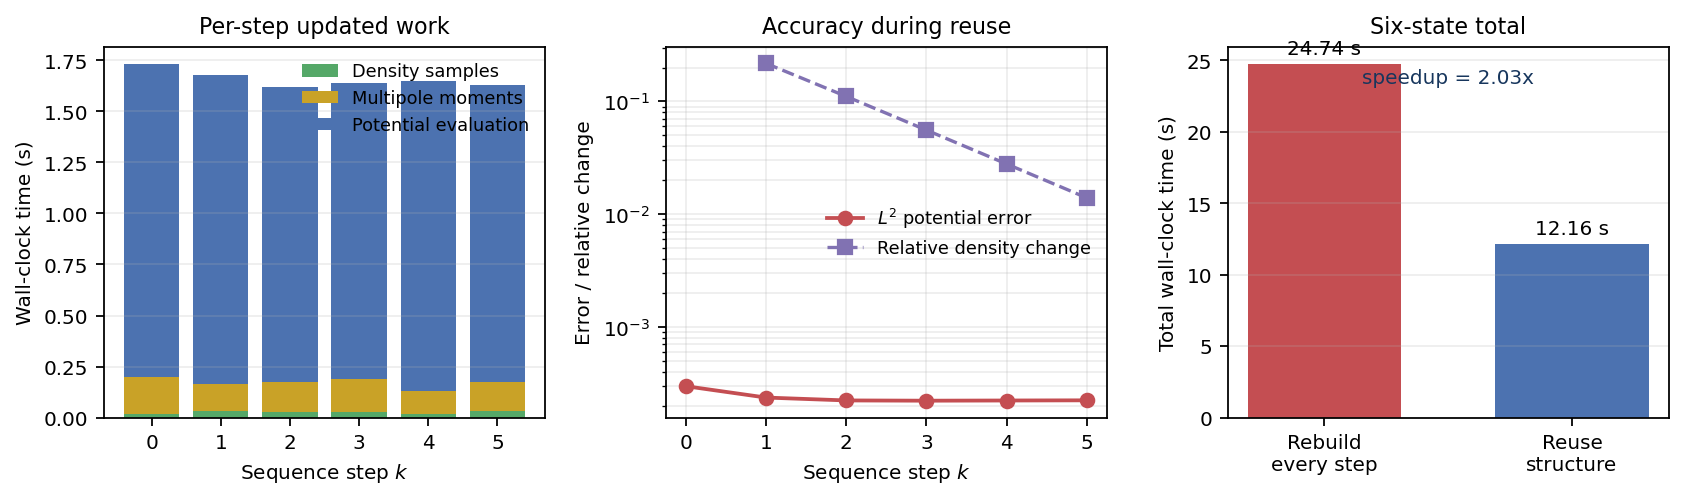
\includegraphics[width=\textwidth]{multirate_reuse_experiment.png}
    \column{0.41\textwidth}
      \small
      六个逐步变化的制造密度：
      \[
        V_k=V_0+\beta_kV_1,
        \qquad \beta_k=0.5(0.5)^k.
      \]
      参数：$n=100\,656$，$p=6$，$P=4$，$\theta=0.5$，128 线程。

      \vspace{0.15cm}
      \begin{tabular}{lrr}
        \toprule
        策略 & 六步时间 & 加速比\\
        \midrule
        每步重建 & 24.739 s & 1.00\\
        结构复用 & 12.160 s & 2.03\\
        \bottomrule
      \end{tabular}

      \vspace{0.25cm}
      两种策略的离散 $L^2$ 误差逐步一致。
  \end{columns}

  \vspace{0.2cm}
  {\footnotesize\color{red}
  边界：这只是实现等价性和时间收益的 proof-of-concept；当前指示子不依赖密度，尚未验证真实 SCF 中的动态触发。}
\end{frame}

\begin{frame}{如何真正接入 KS--SCF：建议的软件接口}
  \small
  \centering
  \begin{tikzpicture}[
      node distance=7mm,
      module/.style={draw=navy,rounded corners=1.8mm,fill=navy!5,minimum width=3.0cm,minimum height=1.05cm,align=center,font=\small\bfseries},
      data/.style={draw=teal,rounded corners=1.8mm,fill=teal!6,minimum width=3.0cm,minimum height=1.05cm,align=center,font=\small},
      arr/.style={-{Latex[length=2mm]},thick,draw=muted}]
    \node[module] (ks) {KS 轨道求解器\\输出 $\psi_i^{(k)},\rho^{(k)}$};
    \node[data,right=of ks] (transfer) {密度转移/采样层\\轨道网格 $\to$ Hartree 网格};
    \node[module,right=of transfer] (tree) {Hartree treecode 状态\\网格、树、列表、GPU 数据};
    \node[data,below=of tree] (vh) {返回 $V_H^{(k)}$\\并计算 $E_H^{(k)}$};
    \node[module,below=of transfer] (control) {误差控制器\\$r_k,e_{H,k},\tau_{H,k}$};
    \draw[arr] (ks)--(transfer);
    \draw[arr] (transfer)--(tree);
    \draw[arr] (tree)--(vh);
    \draw[arr] (vh)--(control);
    \draw[arr] (control)--(ks);
    \draw[arr,dashed,draw=orange] (control)--node[right]{更新命令}(tree);
  \end{tikzpicture}

  \vspace{0.45cm}
  \begin{block}{最小可行版本}
    \centering\small
    不立即改写整个 KS 程序：先定义密度输入、Hartree 势输出、网格更新和计时接口；比较固定间隔与残差触发策略。
  \end{block}
\end{frame}

\begin{frame}{数值验证：四种策略必须在同一体系上比较}
  \begin{columns}[T,onlytextwidth]
    \column{0.53\textwidth}
      \small
      \begin{enumerate}\setlength\itemsep{0.48em}
        \item \textbf{每步重建：}高成本基线；
        \item \textbf{固定间隔：}每 $m$ 步更新一次；
        \item \textbf{残差触发：}拟提出的方法；
        \item \textbf{全程冻结：}揭示过度复用的误差风险。
      \end{enumerate}

      \vspace{0.2cm}
      初始体系建议：H$_2$、H$_2$O、CH$_4$，\par
      再扩展到更大非周期分子。
    \column{0.44\textwidth}
      \begin{block}{统一报告}
        \small
        \begin{itemize}\setlength\itemsep{0.38em}
          \item SCF 步数与最终残差；
          \item 网格/列表更新次数；
          \item $T_{\mathrm{mesh}}$、$T_{\mathrm{list}}$、$T_{\mathrm{moment}}$、$T_{\mathrm{eval}}$；
          \item 总能量、能量差和力误差；
          \item CPU/GPU 总时间与峰值内存。
        \end{itemize}
      \end{block}
  \end{columns}

  \vspace{0.25cm}
  \centering
  \textbf{成功标准：}残差触发法减少结构重建与总时间，同时不增加 SCF 步数且保持最终物理精度。
\end{frame}

\begin{frame}{相对于已有工作的潜在创新点}
  \footnotesize
  \renewcommand{\arraystretch}{0.92}
  \begin{tabularx}{\textwidth}{>{\bfseries\color{navy}}p{0.25\textwidth}X}
    \toprule
    已有基础 & 本工作需要推进的内容\\
    \midrule
    多水平校正 KS 方法 & 不重复求解全部非线性特征值问题\\
    Hartree 与 $V_{\mathrm{xc}}$ 分离处理 & 将自适应 treecode 作为可独立控制的 Hartree 子求解器\\
    波函数/Hartree 多网格 & 从空间网格分离推进到迭代时间尺度分离\\
    TDDFT 空间--时间残差自适应 & 建立 Hartree 专用误差预算与结构更新触发\\
    当前 HGT/treecode & 跨步复用 MAC、局部更新树/列表以及 GPU 常驻数据\\
    \bottomrule
  \end{tabularx}

  \vspace{0.18cm}
  \begin{beamercolorbox}[rounded=true,sep=0.3em,wd=0.96\textwidth]{block body}
    \centering\scriptsize
    仅“隔步更新”不足以构成创新；\\
    还需给出\alert{触发指标、局部更新、物理量控制与端到端收益}。
  \end{beamercolorbox}
\end{frame}

\begin{frame}{关键风险与需要先回答的问题}
  \begin{columns}[T,onlytextwidth]
    \column{0.49\textwidth}
      \begin{block}{数学与数值风险}
        \small
        \begin{itemize}\setlength\itemsep{0.4em}
          \item $e_{H,k}$ 如何低成本且可靠地估计？
          \item 延迟更新是否破坏 SCF 收敛？
          \item 密度转移是否引入新的守恒误差？
          \item 能量足够准确时，原子力是否也足够准确？
        \end{itemize}
      \end{block}
    \column{0.49\textwidth}
      \begin{block}{实现与性能风险}
        \small
        \begin{itemize}\setlength\itemsep{0.4em}
          \item 势求值仍可能主导，复用上限有限；
          \item 网格小改动可能影响大量目标列表；
          \item GPU 不规则近场访问和负载不均；
          \item 轨道网格与 Hartree 网格的数据转移成本。
        \end{itemize}
      \end{block}
  \end{columns}

  \vspace{0.25cm}
  \centering\color{navy}\bfseries
  因此第一阶段先做完整 SCF profiling 和固定间隔基线，再设计复杂触发器。
\end{frame}

\begin{frame}{下一阶段实施路线}
  \small
  \begin{enumerate}\setlength\itemsep{0.48em}
    \item \textbf{接入：}从现有 KS 求解器读取每步轨道或密度，调用当前 Hartree treecode；
    \item \textbf{测量：}记录 SCF 残差、能量、力、网格变化和各阶段时间；
    \item \textbf{基线：}比较每步重建、固定间隔和全程冻结；
    \item \textbf{触发：}实现带上下限、滞回和最大复用步数的残差控制；
    \item \textbf{局部化：}只更新改变的子树、矩和受影响目标的列表；
    \item \textbf{加速：}保持 GPU 静态数据常驻并批量更新密度与矩；
    \item \textbf{扩展：}在基态方法稳定后，再研究 RT--TDDFT 的时间步复用。
  \end{enumerate}

  \vspace{0.35cm}
  \begin{beamercolorbox}[rounded=true,sep=0.45em,wd=0.94\textwidth]{block body}
    \centering
    第一篇工作的合理边界：真实 KS--SCF + 残差触发 + 结构复用 + 能量/力/总时间验证。
  \end{beamercolorbox}
\end{frame}

\begin{frame}{结论与希望讨论的问题}
  \begin{block}{一句话概括新想法}
    \centering
    每一步更新电子密度、矩和 Hartree 势；仅当当前误差预算不再满足时，才更新 Hartree 网格和 treecode 结构。
  \end{block}

  \vspace{0.35cm}
  \small
  \textbf{希望与导师讨论：}
  \begin{enumerate}\setlength\itemsep{0.48em}
    \item 先接入哪一个现有 KSDFT 程序，能够最小成本获得轨道、密度、能量和力？
    \item 第一阶段用 Hartree 能量还是总能量/原子力来校准容许误差？
    \item 当前论文止于单次自适应 Hartree treecode，还是纳入初步 SCF 复用？
    \item 下一篇工作的重点应放在误差控制理论、局部更新，还是 GPU 常驻数据？
  \end{enumerate}

  \vfill
  \centering\Large\bfseries\color{navy}
  从“把单次势算准”转向“把整个自洽过程算得足够准且更快”
\end{frame}

\begin{frame}{参考工作的定位}
  \footnotesize
  \begin{thebibliography}{9}
    \bibitem{Hu2018}
    G. Hu, H. Xie and F. Xu,
    \newblock A multilevel correction adaptive finite element method for Kohn--Sham equation,
    \newblock \emph{J. Comput. Phys.}, 355 (2018), 436--449.

    \bibitem{Hu2023}
    G. Hu, H. Xie and F. Xu,
    \newblock On accelerating a multilevel correction adaptive finite element method for Kohn--Sham equation,
    \newblock \emph{J. Comput. Phys.}, 472 (2023), 111674.

    \bibitem{Kuang2024}
    Y. Kuang, Y. Shen and G. Hu,
    \newblock Towards chemical accuracy using a multi-mesh adaptive finite element method in all-electron DFT,
    \newblock \emph{J. Comput. Phys.}, 518 (2024), 113312.

    \bibitem{Bao2015}
    G. Bao, G. Hu and D. Liu,
    \newblock Real-time adaptive finite element solution of time-dependent Kohn--Sham equation,
    \newblock \emph{J. Comput. Phys.}, 281 (2015), 743--758.
  \end{thebibliography}

\end{frame}

\end{document}
